\section{Method}

\subsection{Overview}

We use DP3~\cite{ze2024dp3} as our base model and extend it with NOCS-based coordinate normalization, directly motivated by UniFolding's~\cite{unifolding2023} demonstrated generalization gains on garment folding. All three provided competition baselines, ACT~\cite{zhao2023act}, Diffusion Policy~\cite{chi2023diffusionpolicy}, and SmolVLA~\cite{smolvla2025}, share the same fundamental limitation: RGB-based visual encoders that encode color and texture rather than geometry, with no explicit mechanism for generalizing to unseen garment styles. Our approach addresses this at two levels. DP3 replaces RGB with point clouds, forcing the policy to reason about shape and structure. NOCS then normalizes that geometric representation into a canonical coordinate space so that the same geometric features can be recognized across garments of different sizes and proportions.

\begin{figure*}[t]
    \centering
    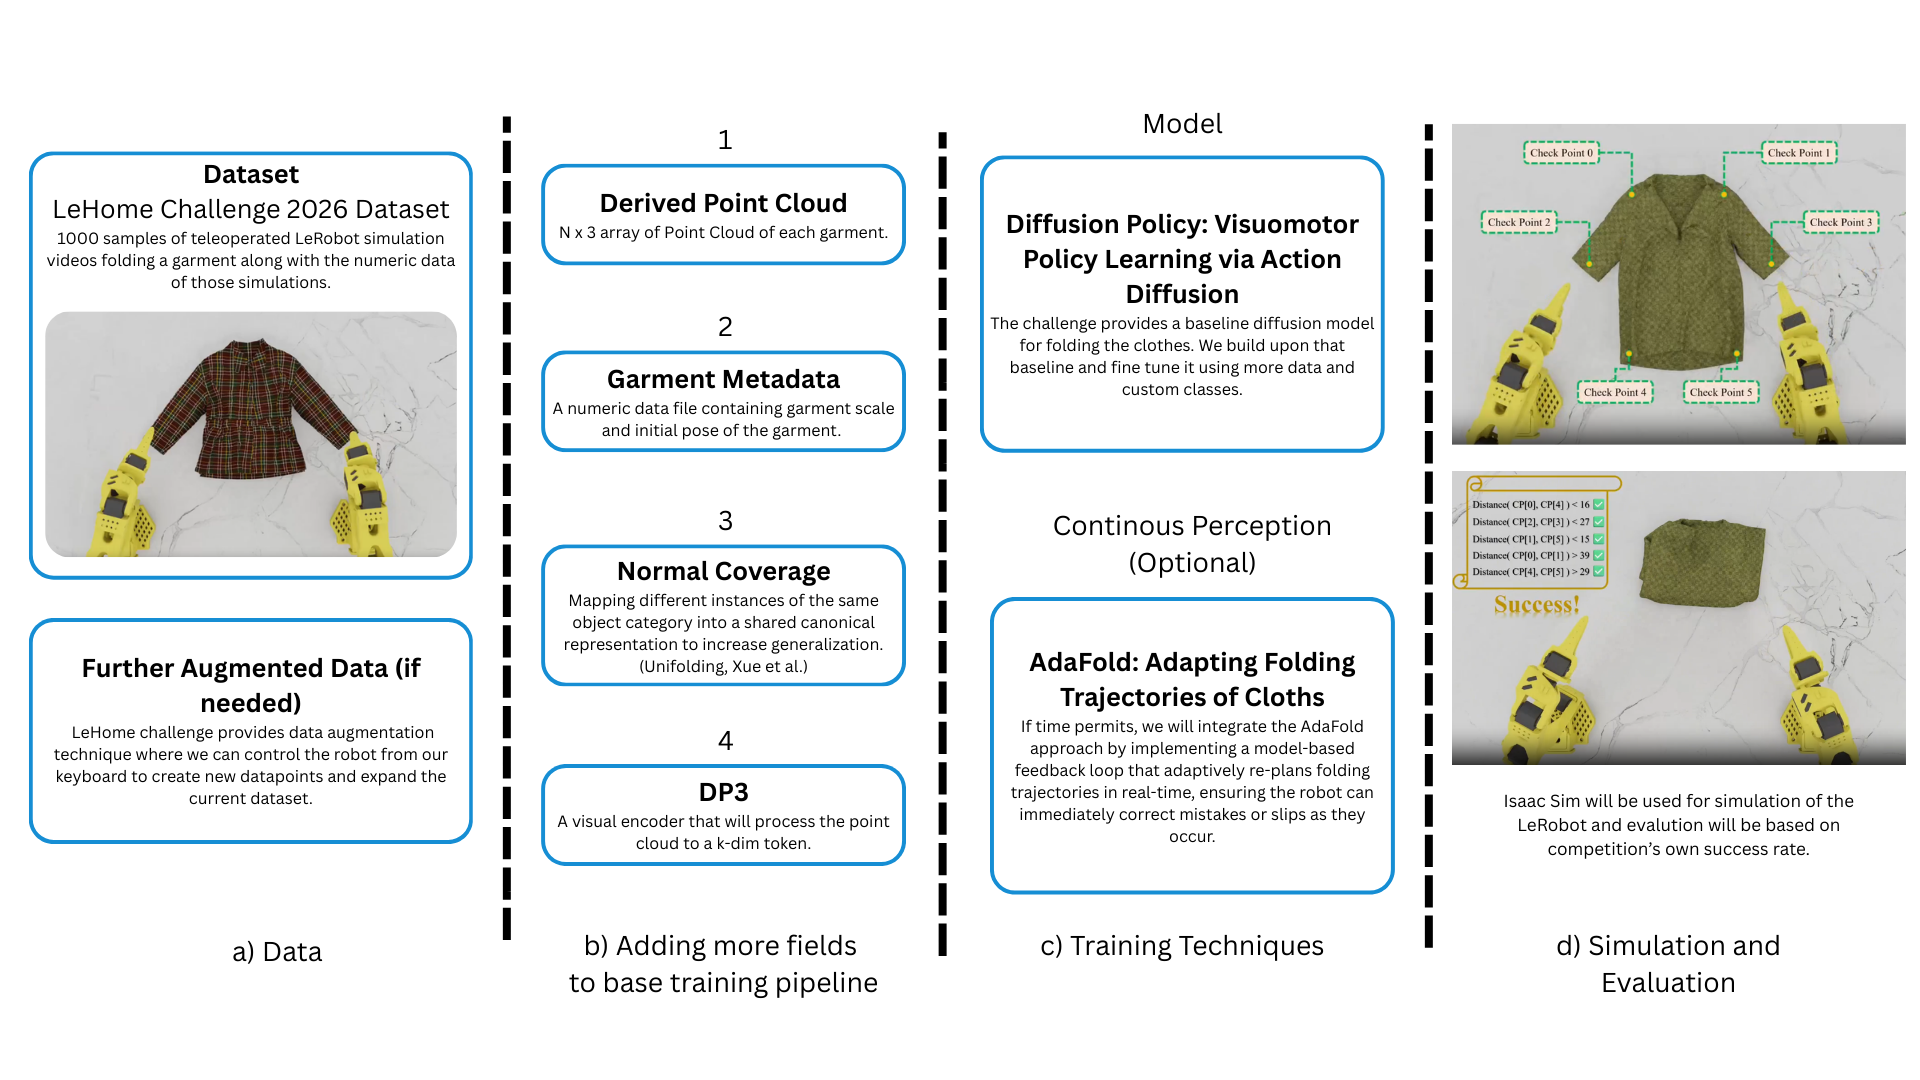
\includegraphics[width=\textwidth]{figs/pipeline.png}
    \caption{Overview of our approach. (a) Training data consists of the LeHome dataset with depth recordings and garment metadata. (b) We augment the base training pipeline with derived point clouds, garment metadata conditioning, NOCS normalization, and a point cloud encoder. (c) We build on Diffusion Policy as our base model, extended with our geometric visual representation. (d) Evaluation is performed in IsaacSim using the competition's success rate metric based on cloth mesh vertex positions.}
    \label{fig:pipeline}
\end{figure*}

\subsection{Base Model: DP3}

We choose DP3 over the provided baselines because its architecture is built around point cloud representations, meaning our NOCS contribution integrates cleanly rather than requiring significant restructuring. Its open-source implementation provides a working starting point for both the point cloud encoder and the diffusion action head~\cite{ze2024dp3}. It works with as few as 10 demonstrations, making our 250-demo budget more than sufficient. Its generalization advantage over RGB-based policies, demonstrated across appearance, instance, spatial, and view dimensions on rigid objects, directly targets the unseen garment evaluation criterion of our competition. We use Diffusion Policy as our primary comparison baseline since it has been tested on shirt folding with a similar demo count and represents the strongest RGB-based reference point.

At inference time, depth images from the simulation are converted to point clouds online using camera intrinsics, processed through DP3's MLP encoder, and passed to the diffusion action head to produce joint angle targets for both arms.

\subsection{NOCS Normalization for Garment Generalization}

Different garment instances of the same category, say two long-sleeved shirts, can vary significantly in size, proportions, and the exact positions of their geometric landmarks. A policy that reasons in raw physical coordinates has to relearn these relationships for every new garment it encounters. NOCS addresses this by mapping all instances of a category into a shared canonical coordinate space, so that the same location on a shirt sleeve always corresponds to the same normalized coordinate regardless of which specific shirt is being folded.

We apply this principle to our point cloud representation. Rather than feeding the policy raw 3D point positions from the simulation, we normalize the point cloud into a canonical space defined by consistent geometric landmarks on the garment, such as collar corners, sleeve tips, and hem edges. These landmarks are semantically consistent across all garment styles within a category, meaning the normalization generalizes to unseen instances. The policy then learns manipulation strategies in this canonical space, which transfer to new garments without retraining because the geometric relationships it learned remain valid after normalization.

This is the same mechanism behind UniFolding's cross-garment generalization, which we adapt from their pick-and-place action space into DP3's continuous joint trajectory framework.

\subsection{Garment Metadata Conditioning}

In addition to the point cloud input, we condition the policy on garment scale and initial pose from the dataset's \texttt{garment\_info.json} metadata, which is already available per episode at zero additional engineering cost. This provides the policy with explicit information about garment size and starting configuration, which varies across styles and episodes.

\subsection{Dataset and Implementation}

We use the official LeHome dataset hosted on HuggingFace, accessed through the raw recordings which include depth data (\texttt{observation.top\_depth}) omitted from the merged datasets. We re-record a subset of demonstrations with the modified pipeline to capture keypoint positions needed for NOCS normalization. Our implementation builds on the DP3 codebase~\cite{ze2024dp3} and the UniFolding codebase~\cite{unifolding2023}, integrated with the competition's custom \texttt{BasePolicy} interface.
